\section{Support Vector Machine}
\subsection{Training phase}
After having extracted the aforesaid features, as indicated in the followed paper \cite{paper}, a support vector machine (SVM) has been used in order to classify unknown images.\\
The kernel used is of the linear kind and the training phase has been structured as follows :
\begin{itemize}
    % \item the path of every image, recaptured and single captured ones, has been extracted and stored in different lists one for each camera model;
    % \item at this point a random split has been performed as specified in the aforesaid paper:
        % \begin{itemize}
            % \item concerning the single captured images, $15$ images are kept for training purposes;
            % \item for the recaptured examples, the training set's size is set to $3$.
        % \end{itemize}
        % At the end of this point, all the training and test lists of each camera are put together obtaining two lists respectively conatining training and test samples' paths. \\
        % More specifically, four lists have to be obtained : 
        % \begin{enumerate}
            % \item training list for recaptured images with with $3$ elements;
            % \item training list for single captured list woth $15$`';
            % \item test list for recaptured images;
            % \item test list for single captured images.
        % \end{enumerate}
    \item paths of images used for training purposes are stored in two separated lists, both for recaptured and single captured;
    \item pre-computed dictionaries are loaded;
    \item iteratively, for each element within the two lists : 
        \begin{itemize}
            \item the corresponding already calculated list of $Q_i$ is loaded;
            \item the features (approximation error $E_d$ and average line spread function width $\lambda_{avg}$) are computed and saved within a common Pandas DataFrame [\textbf{Picture} \ref{fig:table_csv}] organized in columns as follows:
          \begin{itemize}
              \item first column : it's composed by integer indexes;
              \item second column : it's formed, cell by cell, by the path of a specific processed image;
              \item third column : it contains the true label of a specific image;
              \item fourth column :  it displays the computed values of $\lambda_{avg}$ for the corresponding image;
              \item fifth and last column : element-wise, it showcases approximation errors.
          \end{itemize}
        \end{itemize}
          It's worth mentioning that the previously calculated $Q_i$ and dictionaries are loaded in order to save some computational power;
    \item at the end, a unified csv table made of training samples including both recaptured and single captured values, is used to train the SVM. Once the fitting has finished, the resulting model is saved in preparation for future predicting operations.
\end{itemize}

\begin{figure}[h!]
    \centering 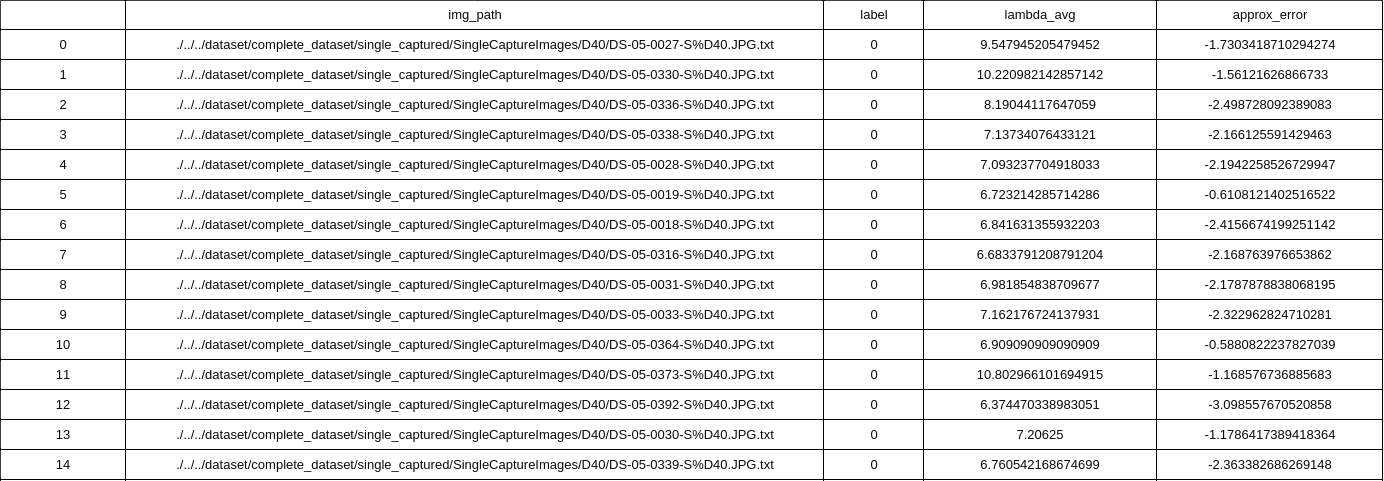
\includegraphics[width=\textwidth]{Images/table.png}
    \caption{Pieces of Panda DataFrame table in .csv file format.}
    \label{fig:table_csv}
\end{figure}
